% !TEX spellcheck=it_IT
\documentclass[11pt,a4paper,notitlepage]{report}
\usepackage[utf8]{inputenc}
\usepackage{amssymb}
\usepackage{amsthm}
\usepackage{mathtools}
\usepackage{makeidx}
\usepackage{booktabs}
\usepackage{hyperref}
\usepackage{wrapfig}
\usepackage{float}

\let\numberset\mathbb
\newcommand{\N}{\numberset{N}}
\newcommand{\Z}{\numberset{Z}}
\newcommand{\Q}{\numberset{Q}}
\newcommand{\R}{\numberset{R}}
\newcommand{\C}{\numberset{C}}
\newcommand{\U}{\numberset{U}}
\newcommand{\I}{\numberset{I}}
\newcommand{\PP}{\numberset{P}}
\newcommand{\CC}{\complement}
\newcommand{\dom}{\text{dom }}
\newcommand{\im}{\text{Im }}

\hypersetup{
  pdfauthor   = {Riccardo Cereghino},
  pdftitle    = {Calculus I}
}

\begin{document}
\begin{titlepage}
	\title{Calculus I}
	\author{Riccardo Cereghino \\ S4651066}
	\maketitle
	\tableofcontents
\end{titlepage}

\chapter{Notazione}
\section{Insiemi}
\begin{itemize}
	\item $\emptyset = $ Insieme vuoto
	\item $\N = \{0,1,2,3...\} = $ Naturali
	\item $\Z = \{...-3,-2,-1,0,1 ,2,3...\} = $ Relativi
	\item $\Q = \left\{ \frac{n}{m} \middle| n \in \Z , m \in \Z , m \neq 0 \right\} = $ Razionali
	\item $\R = $ Reali
\end{itemize}

\section{Logica}
\begin{itemize}
	\item $| $ tale che
	\item $ \Rightarrow $ implica
	\item $ \Leftrightarrow $ se e solo se
	\item $ \forall $ per ogni
	\item $ \exists $ esiste
	\item $ \nexists $ non esiste
	\item $ \in $ appartiene
	\item $ \notin $ non appartiene
\end{itemize}

\section{Operazioni tra insiemi}
\begin{itemize}
	\item A sottoinsieme di B
		\[A \subseteq  B\]
		\[\forall x \in A \Rightarrow x \in B\]
	\item A sottoinsieme proprio
		\[A \subsetneqq  B\]
		\[
			\begin{cases}
				\forall x \in A \Rightarrow x \in B \\
				\exists x \in B | x \notin A
  			\end{cases}
  		\]
  	\item Intersezione
  		\[A \cap B = \left\{ x \in X \middle| x \in A, x \in B\right\}\]
  	\item Unione
  		\[A \cup B = \left\{ x \in X \middle| x \in A or x \in B\right\}\]
  	\item Differenza insiemistica
  		\[A \diagdown B = \left\{ x \in X \middle| x \in A, x \notin B\right\}\]
  	\item Complementare
  		\[A^C = \left\{ x \in X \middle| x \notin A \right\}\]
\end{itemize}

\section{Prodotto cartesiano}
Assegnati due numeri reali $a, b, a < b$, si definiscono intervalli gli insiemi seguenti:
\[A\times B = \left\{ (x,y) \middle| x\in A, y\in B\right\}\]
Coppia ordinata: $(1,3) \neq (3,1)$
\subsection{Intervalli}
\[[a,b] = \left\{ x\in \R \middle| a \leq x \leq b \right\}\]
\[(a,b) = \left\{ x\in \R \middle| a < x < b \right\}\]
\[[a,b) = \left\{ x\in \R \middle| a \leq x < b \right\}\]
\[(a,b] = \left\{ x\in \R \middle| a < x \leq b \right\}\]

\[[a,+\infty) = \left\{ x\in \R \middle| x \geq a \right\}\]
\[(a,+\infty) = \left\{ x\in \R \middle| x > a \right\}\]
\[(-\infty,b] = \left\{ x\in \R \middle| x \leq b \right\}\]
\[(-\infty,b) = \left\{ x\in \R \middle| x < b \right\}\]
\[(-\infty,+\infty) = \R\]

\section{Proprietà delle operazioni tra numeri reali}
\[x,y,z \in \R\]
\begin{itemize}
	\item Associativa
		\[(x+y)+z=x+(y+z)=x+y+z \]
		\[(xy)z=x(yz)=xyz \]
	\item Commutativa
		\[x+y=y+x\]
		\[xy=yx\]
	\item Distributiva
		\[x(y+z)=xy+xz\]
	\item Esistenza elemento neutro
		\[x+0=x\]
		\[1x=x\]
	\item Esistenza dell'universo
		\begin{enumerate}
			\item \[\forall x \in \R \quad \exists !y=-x \in \R | x+(-x)=0\]
			\item \[\forall x \in \R \quad x \neq 0 \quad \exists !y=\frac{1}{x} \in \R | x\frac{1}{x}=1 \]
		\end{enumerate}
	\item Relazione d'ordine totale
		\[x,y,z \in \R\]
		\[
		\begin{cases}
			x<y \quad oppure\\
			x=y \quad oppure\\
			x>y
		\end{cases}
		\]
	\item Transitività
		\[x,y,z \in \R\]
		\[(x<y) \cap (y<z) \Rightarrow (x<z)\]
	\item Compatibilità con la somma
		\[x,y,z \in \R\]
		\[x<y \Rightarrow x+z<y+z\]
	\item Compatibilità con il prodotto
		\[x,y,z \in \R\]
		\[x<y \cap z>0 \Rightarrow xz<yz\]
		\[x<y \cap z<0 \Rightarrow xz>yz\]
\end{itemize}

\section{Geometria}
\subsection{Circonferenza}
Dato il centro di una circonferenza $C=(x_c,y_c)$
Si esprime l'equazione della circonferenza nella forma:
\[(x-x_c)^2+(y-y_c)^2=r^2\]

\[x^2+y^2+\alpha x+ \beta y +\gamma =r^2\]
Per cui se $O=(0,0)$
\[x^2+y^2=r^2\]


\paragraph{Forma canonica:}
\[\alpha = -2x_c \quad \beta = -2y_c \quad \gamma = x_c^2 + y_c^2 - r^2\]
\[x^2+y^2+\alpha x+ \beta y +\gamma =r^2\]

Da cui calcolare centro e raggio:
\[C=\left(-\frac{\alpha}{2}, -\frac{\beta}{2}\right); \quad r=\sqrt{\frac{\alpha^2}{4}+\frac{\beta^2}{4}-\gamma}\]

\subsection{Ellisse}
Equazione dell'ellisse (con centro nell'origine degli assi)
\[\frac{x^2}{a^2}+\frac{y^2}{b^2} \qquad a\neq 0 , b\neq 0\]




\chapter{Funzioni}
\section{Il concetto di funzione}
\textbf{Definizione:} una funzione $f: A \rightarrow \R$ dove $A \subseteq \R$ è una legge che assegna ad ogni $x\in A$ uno ed un solo valore $y=f(x) \in \R$

\textit{Nota:} in questo caso, i valori di $A$ sono chiamati variabile indipendente $(x)$, mentre  $\R$ è la variabile dipendente $y=f(x)$

\textit{Nota:} inoltre definiamo $A=dom \quad f$ come il dominio della funzione.

\textbf{Definizione:} Il grafico di $f$:
	\[f=\left\{ (x,y) \in \R^2 \middle| x \in A, y=f(x) \right\}\]

\textbf{Definizione:} L'immagine di $f$, Im f:
	\[f(A)=\left\{ f(x) \in \R \middle| x \in A \right\}\]

\section{Operazioni tra funzioni}
Date due funzioni $f:A\rightarrow \R \qquad g:B\rightarrow \R$
\begin{description}
	\item[Somma e differenza:] $(f+g)(x)=f(x)+g(x) \qquad dom(f+g)=A\cap B$
	\item[Prodotto:] $(fg)(x)=f(x)g(x) \quad dom(fg)=(A\cap B)$
	\item[Rapporto:] $(\frac{f}{g})(x)=f(x)g(x) \quad dom(\frac{f}{g})=\{x\in \R | x\in A, x\in B, g(x) \neq 0\}$
	\item[Reciproco:] $\frac{1}{f}(x)=\frac{1}{f(x)}=[f(x)]^{-1} \quad dom(\frac{1}{f})={x\in A | f(x) \neq 0}$
\end{description}

\subsection{Nomenclatura}
Data una funzione $f: A \rightarrow \R , \quad y=f(x)$
\begin{itemize}
	\item $f$ è detta \textbf{iniettiva} se $\forall y_0 \in \R , f(x)=y_0$ ha al più una soluzione.
	\item $f$ è detta \textbf{surgettiva} se $\forall y_0 \in \R , f(x)=y_0$ ha almeno una soluzione.
	\item $f$ è detta \textbf{bigettiva} se $\forall y_0 \in \R , f(x)=y_0$ ha una ed una sola soluzione, ovvero se la funzione è sia iniettiva che surgettiva.
\end{itemize}

\subsubsection{Osservazioni}
\begin{enumerate}
	\item $f$ è surgettiva se e solo se $IM f=\R$
	\item $f$ è iniettiva se e solo se $y_0 \in IM f, f(x)=y_0$ ha al più una soluzione.
\end{enumerate}

Data una funzione $f: A \rightarrow \R , \quad y=f(x)$ sono fatti equivalenti:
\begin{itemize}
	\item $f$ è iniettiva
	\item $\forall x_1, x_2 \in A \cap x_1 \neq x_2$ allora $f(x_1)\neq f(x_2)$
	\item dati $x_1,x_2 \in A | f(x_1)=f(x_2)$ allora $x_1=x_2$
\end{itemize}


\section{Funzioni reali di variabile reale}
\subsection{Funzioni pari e dispari}
Data una funzione $f: A \rightarrow \R , \quad y=f(x)$, $\forall x\in A \quad -x\in A$ f è detta:
\[f(-x)= \begin{cases}
	f(x) \qquad pari\\
	-f(x) \qquad dispari
\end{cases}
\]

\subsection{Funzioni monotone}
Data una funzione $f: A \rightarrow \R , \quad y=f(x)$
\begin{itemize}
	\item $\forall x_1, x_2 \in A \quad x_1<x_2$ f è detta:
	\[\begin{cases}
		f(x_1) \leq f(x_2) \qquad crescente\\
		f(x_1) \geq f(x_2) \qquad decrescente
	\end{cases}
	\]
	\item $\forall x_1, x_2 \in A \quad x_1<x_2$ f è detta:
	\[\begin{cases}
		f(x_1) < f(x_2) \qquad strettamente crescente\\
		f(x_1) > f(x_2) \qquad strettamente decrescente
	\end{cases}
	\]
\end{itemize}


\section{Traslazioni, dilatazioni e riflessioni}
Data una funzione $f: A \rightarrow \R , \quad y=f(x)$:
\begin{description}
	\item[Traslazioni:] $x_0 > 0, \quad y_0 \in \R$
		\[g(x)=f(x-x_0) \text{ Traslazione verso destra}\]
		\[g(x)=f(x+x_0) \text{ Traslazione verso sinistra}\]
		\[g(x)=f(x)+y_0 \text{ Traslazione verso l'alto}\]
		\[g(x)=f(x)-y_0 \text{ Traslazione verso il basso}\]
	\item[Dilatazioni:] $a>0$
		\[g(x)=f(\frac{x}{a}) \text{ Dilata su asse x}\]
		\[g(x)=a\times f(x) \text{ Dilata su asse y}\]
	\item[Riflessioni:]
		\[g(x)=f(-x) \text{ Riflette su asse }y\]
		\[g(x)=-f(x) \text{ Riflette su asse }x\]
		\[g(x)=-f(-x) \text{ Riflette rispetto l'origine}\]
\end{description}


\subsubsection{Osservazioni}
Se $f(x)$ è dispari e $0 \in \text{dom f}$
\[f(0)=f(-0)=-f(0)\Rightarrow f(0)=0\]
\newline
Se $n \in \N, n \geq 1$
\[f(x)=x^n= \underbrace{x \times \dots \times x}_{\textbf{n volte}}\]
\begin{itemize}
	\item se $n$ è pari, $f$ è pari
	\item se $n$ è dispari, $f$ è dispari
\end{itemize}

\section{Simmetrie, traslazioni, compressioni e dilatazioni di grafici.}
Data una funzione $f: A \rightarrow \R , \quad y=f(x)$:
\begin{description}
	\item[Traslazioni:] $x_0 > 0, \quad y_0 \in \R$
		\[g(x)=f(x-x_0) \text{ Traslazione verso destra}\]
		\[g(x)=f(x+x_0) \text{ Traslazione verso sinistra}\]
		\[g(x)=f(x)+y_0 \text{ Traslazione verso l'alto}\]
		\[g(x)=f(x)-y_0 \text{ Traslazione verso il basso}\]
	\item[Dilatazioni:] $a>0$
		\[g(x)=f(\frac{x}{a}) \text{ Dilata su asse x}\]
		\[g(x)=a\times f(x) \text{ Dilata su asse y}\]
	\item[Riflessioni:]
		\[g(x)=f(-x) \text{ Riflette su asse }y\]
		\[g(x)=-f(x) \text{ Riflette su asse }x\]
		\[g(x)=-f(-x) \text{ Riflette rispetto l'origine}\]
\end{description}

\section{Funzione composta}
Date due funzioni $f:A\rightarrow \R \qquad g:B\rightarrow \R$
\[g(y)=g(f(x))=g\circ f(x) \qquad \text{dom }g\circ f(x)=\{x\in A \cap f(x) \in \qquad \text{se n dispari} \\ B\}\]

\section{Funzione inversa e sue proprietà.}
Data una funzione iniettiva $f:A\rightarrow \R$
\[\forall y \in f=f(A), \exists ! x\in A | f(x)=y\]
Da cui si ricava che:
\[x=f^{-1}(y) \qquad f^{-1}: B\rightarrow \R \qquad B=Im f\]
\subsection{Costruire l'inverso di f}
\begin{enumerate}
	\item Determinare $Im f=B$ e $dom f^{-1}=B$
	\item $y \in B$ determiniamo $x \in A | f(x)=y$
	\item $x=f^{-1}(y)$
	\item $y=f^{-1}(x) \qquad x\rightleftarrows y$
\end{enumerate}
Il grafico di $y=f^{-1}(x)$ è simmetrico rispetto alla bisettrice $x=y$ della funzione $y=f(x)$
\subsubsection{Osservazioni}
\[f(f^{-1}(y)) = y \qquad \forall y \in dom^{f^{-1}}=Im f \]
\[f^{-1}(f(x)) = x \qquad \forall x \in dom f = Im f^{-1}\]
Inoltre $f$ è invertibile se e solo se è iniettiva o surgettiva, da cui: 
\[g^{-1}:Im f \rightarrow \R\]

\section{Funzioni elementari}
\subsection{Polinomi}
\[f(x)=a_0+a_1 x + \dots + a_n x^n =\displaystyle\sum_{k=0}^{n} a_k x^k \]
\[a_0, a_1, \dots, a_n \in \R \text{ Coefficienti}\qquad a_n \neq 0 \text{ n è il grado del polinomio}\]

Per cui:
\[n=1 \qquad y=a_0+a_1 x \quad \text{Rette}\]
\[n=2 \qquad y=a_0+a_1 x + a_2 x^2 \quad \text{Parabole}\]
\subsection{Potenze}
Fissato un esponente $a \in \R$ la funzione potenza è:
\[f(x)=x^a\]
la cui definizione e dominio dipendono dal valore dell’esponente a.
\begin{itemize}
\item $a=n \in \N$
\[f(x)=x^n= \underbrace{x \times \dots \times x}_{\textbf{n volte}} \qquad \dom f=\R \qquad \im f= 
\begin{cases}
		\R \qquad \text{se n dispari} \\
		[0,+\infty )  \qquad \text{se n pari } n \neq 0 \\
		\{0\}  \qquad n = 1
\end{cases}\]

\item $a=-n\in \Z , n\in \N ,n \geq 1$
\[f(x)=x^{-n}=\frac{1}{x^n} \qquad \dom f = \R \backslash \{0\} \qquad \im f=
\begin{cases}
		\R \backslash \{0\} \qquad \text{n dispari} \\
		(0,+\infty )  \qquad \text{n pari }
\end{cases}
\]
\item $a=\frac{1}{n} \in \Z , n\in \N ,n \geq 2$
\[f(x)=x^{\frac{1}{n}}=\sqrt[n]{x} \qquad 
\dom f = 
\begin{cases}
		\R \qquad \text{n dispari} \\
		[0,+\infty )  \qquad \text{n pari }
\end{cases}
\qquad \im f=
\begin{cases}
		\R \qquad \text{n dispari} \\
		[0,+\infty) \qquad \text{n pari }
\end{cases}
\]

\item $a=\frac{m}{n} \in \Q , n\in \N ,n \geq 1 , m \in \Z$
\[f(x)=x^{\frac{m}{n}}=\sqrt[n]{m} \qquad 
\dom f = (0,+\infty)
\qquad \im f=(0,+\infty)\]

\item $a \in \R$
\[f(x)=x^a=
\begin{cases}
	\text{sup}\{x^q | q \in \Q , q \leq a\} \quad x \geq 1 \\
	\text{inf} \{x^q | q\in \Q , q \leq a\} \quad 0 < x < 1
\end{cases}
\qquad
\dom f = (0, + \infty)
\qquad
\im f = (0, + \infty)
\]


\end{itemize}

\begin{wrapfigure}{r}{0.65\textwidth}
  \begin{center}
    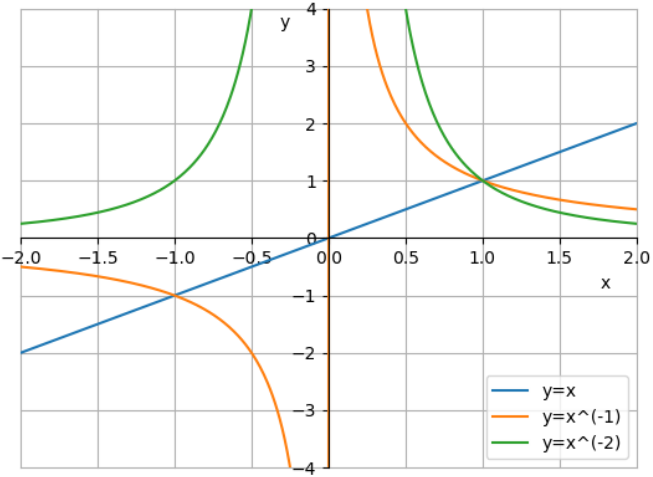
\includegraphics[width=0.65\textwidth]{images/potenze.png}
  \end{center}
  \caption{Potenze}
\end{wrapfigure}

Osserviamo che:
\begin{itemize}
	\item $f(0)=0$
	\item $f(1)=1$
	\item se $n$ pari $f$ è pari
	\item se $n$ dispari $f$ è dispari
\end{itemize}

\subsubsection{Proprietà delle potenze}
\begin{itemize}
\item $x^{n+m}=x^n x^m$
\item $(x^n)^m=x^{nm}$
\end{itemize}

\paragraph{Osservazioni}
\[f(x)=x^0=1 \quad \forall x \in \R\]
\[0^0=1\]

\paragraph{Dimostrazioni}

\[x^{n+m}= \underbrace{x \times \dots \times x}_{\text{n+m volte}}=\underbrace{(x \times \dots \times x)}_{\text{n volte}}\times \underbrace{x \times \dots \times x}_{\text{m volte}}=x^{n+m}\]

\[(x^{n})^m= \underbrace{x^n \times \dots \times x^n}_{\text{m volte}}\]

\[x^n=x^{n+0}=x^n x^0 \qquad x\neq 0\]
\[x^0 = 1 \quad \forall x \in \R\]

\subsection{Esponenziale}
Fissata la base $a>0$ con $a \neq 1$, la funzione esponenziale è
\[f(x)=a^x \qquad \dom f = \R \qquad \im f = (0,+\infty)\]
Se si sceglie come base il numero di Nepero $e=2.71828\dots > 1$, la funzione esponenziale si denota:
\[f(x)=e^x=\exp x\]

\subsubsection{Proprietà}
\begin{enumerate}
	\item se $a>1$, allora la funzzione $a^x$ è strettamente crescente
	\item se $0<a<1$, allora la funzione $a^x$ è strettamente decrescente
	\item se $0<a<b$ con $a,b \neq 1$
	\[\begin{cases}
		a^x<b^x \qquad x>0 \\
		a^x > b^x \qquad x<0
	\end{cases}\]
	\item valgono le seguenti proprietà:
	\begin{itemize}
	\item $a^0=1$
	\item $a^1=a$
	\item $a^{x_1+x_2}=a^{x_1+x_2} \qquad x_1,x_2 \in \R$
	\item $a^{-x}=(\frac{1}{a})^x \qquad x \in \R$
	\item $(a^x)^b = a^{bx} \qquad x,b \in \R$
	\end{itemize}
\end{enumerate}

\begin{figure}[H]
  \centering
    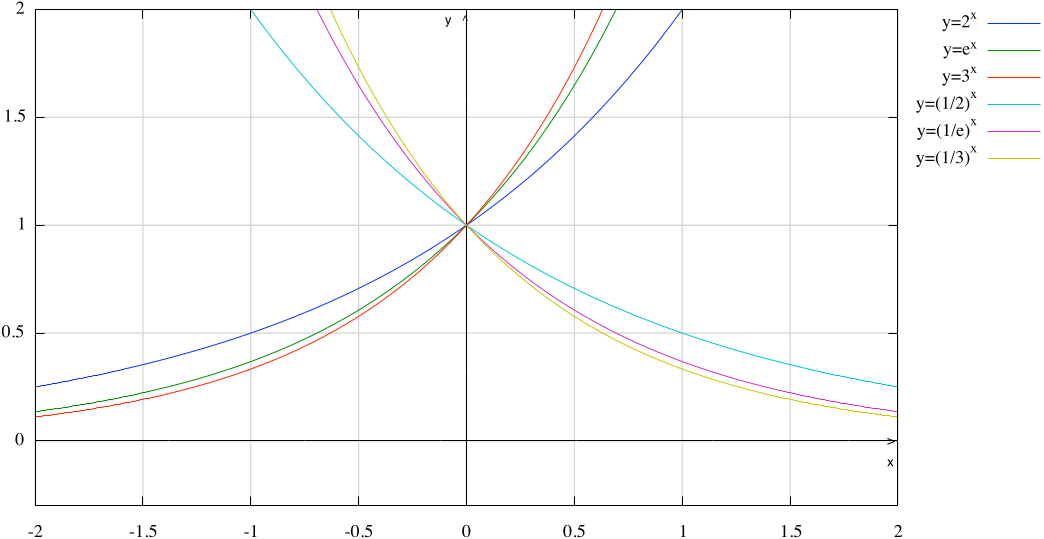
\includegraphics[width=1\textwidth]{images/esponenziali.png}
  \caption{Esponenziali}
\end{figure}

\subsection{Logaritmo}
Fissata la base $a>0$ con $a\neq 1$, la funzione logaritmo
\[f(x)=\log_a x \qquad \dom f = (0,+\infty) \qquad \im f = \R\]
è definita come la funzione inversa della funzione esponenziale $a^x$. Se si sceglie come base il numero di Nepero \textit{e}, il logaritmo si denota:
\[f(x)=\log_e = \log x = \ln x\]

\begin{enumerate}
	\item se $a>1$, allora la funzione $\log_a x$ è strettamente crescente
	\item se $0<a<1$, allora la funzione $\log_a x$ è strettamente decrescente
	\item se $0<a<b$ con $a,b\neq 1$
	\[\begin{cases}
	\log_a x > \log_b x \qquad se x>1 \\
	\log_a x < \log_b x \qquad se 0<x<1 \\
	\end{cases}\]
	\item valgono le seguenti proprietà:
	\begin{itemize}
		\item $\log_a a^x = x \qquad x>1$
		\item $a^{\log_a x}=x \qquad x>0$
		\item $\log_a 1 = 0$
		\item $\log_a a = 1$
		\item $\log_a (x_1 x_2)= \log_a x_1 + \log_a x_2 \qquad x_1,x_2 > 0$
		\item $\log_a (\frac{x_1}{x_2})=\log_a x_1 - \log_a x_2 \qquad x_1,x_2 > 0$
		\item $\log_a x^b = b \log_a x \qquad x>0, b \in \R$
		\item $\log_a x= \frac{\log_b x}{\log_b a}=\frac{\ln x}{\ln a}\qquad x>0,b>0,b\neq 1$
		\item $a^x = e^{(\ln a)x} \qquad x\in \R, a>0, a \neq 1$
	\end{itemize}
\end{enumerate}
\begin{figure}[H]
  \centering
    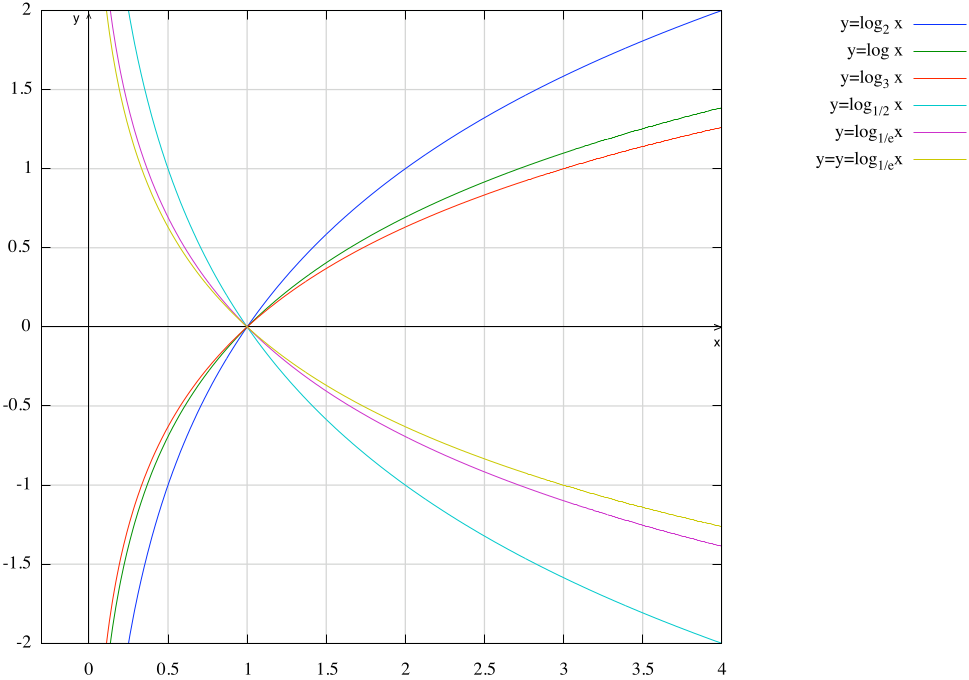
\includegraphics[width=1\textwidth]{images/logaritmi.png}
  \caption{Logaritmi}
\end{figure}

\section{Funzioni trigonometriche}
Una funuone $f:\R \in \R$ è detta periodica di periodo $T$, $T>0$ se:
\[f(x+T)=f(x) \forall x \in \R\]
La caratteristica fondamentale delle funzioni periodiche è che i suoi valori si ripetono dopo intervalli di ampiezza $T$.

\subsection{Le funzioni seno e coseno}
Sia $\gamma$ una circonferenza di raggio $1$ (detta circonferenza goniometrica) il cui centro $O$ è anche l'origine di un sistema di assi cartesiani e sia $A$ il punto $(1,0)$.
Partendo da $A$ percorriamo la circonferenza in senso antiorario oppure in senso orario.
Sia $x$ un numero reale, denotiamo con $P_x$ il punto su $\gamma$ che si ottiene percorrendo la circonferenza a partire dal punto $A$ per un arco di lunghezza $|x|$, in senso antorario se $x \geq 0$, oppure in senso orario se $x<0$.
Il punto $P_x$ individua un angolo nel piano avente vertice $O$ e delimitatio dalle semirette nel piano uscenti da $O$ e passanti per $A$ e per $P_x$.
Il numero reale $x$ rappresenta la misura dell'angolo in radianti.

\begin{wrapfigure}{r}{0.40\textwidth}
  \begin{center}
    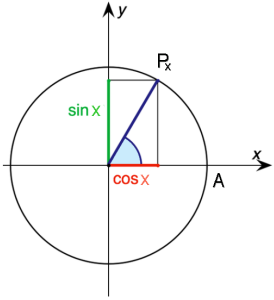
\includegraphics[width=0.40\textwidth]{images/circonferenza.png}
  \end{center}
  \caption{Circonferenza goniometrica con seno e coseno}
\end{wrapfigure}


Osserviamo che l'incremento della lunghezza $x$ di $2\pi$ corrisponde a compiere un intero giro sulla circonferenza in senso antiorario ritornando al punto $P_x$ (così come decrementare di $2\pi$ la lunghezza $x$). Quindi si ha:
\[P_{x\pm k2\pi}=P_x \qquad \forall x \in \R, k \in \N\]

\paragraph{Simmetria}
Indichiamo con $\cos x$ e con $\sin x$ rispettivamente l'ascissa e l'ordinata del punto $P_x$. Le funzioni $y=\cos x$ e $y=\sin x$ sono definite su $\R$ a valori nell'intervallo $[-1,1]$, sono periodiche di minimo periodo $2\pi$ e soddisfano la relazione:
\[\sin^2 x + \cos^2 x = 1\]

\paragraph{Monotonia} Per la periodicità di seno e coseno ci basta studiarne le proprietà nell'intervallo $[0,2\pi]$. Dalle definizioni segue subito che la funzione seno è dispari e la funzione coseno è pari; inoltre la funzione coseno è strettamente decrescente in $[0,\pi]$ e strettamente crescente in $[\pi,2\pi]$. La funzione seno è strettamente crescente in $[0,\frac{\pi}{2}] \cup [\frac{3}{2}\pi,2\pi)$ e strettamente decrescente in $[\frac{\pi}{2},\frac{3}{2}\pi]$.

\begin{figure}[H]
  \centering
    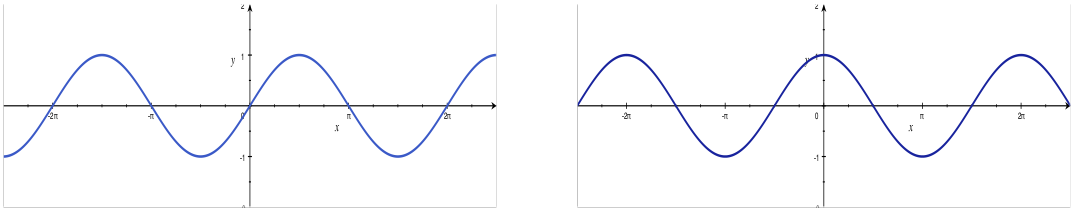
\includegraphics[width=1\textwidth]{images/senocoseno.png}
  \caption{Grafico delle funzioni: seno (sinistra) e coseno (destra)}
\end{figure}

\subsubsection{Formule trigonometriche}
\paragraph{Formule di addizione e sottrazione}
\[\sin(\alpha\pm\beta)=\sin(\alpha)\cos(\beta)\pm\cos(\alpha)\sin(\beta)\]
\[\cos(\alpha\pm\beta)=\cos(\alpha)\cos(\beta)\mp\sin(\alpha)\sin(\beta)\]
\paragraph{Formule di duplicazione}
\[\sin(2x)=2\sin x\cos x\]
\[\cos(2x)=2\cos^2 x - 1\]
\paragraph{Formule di potenza}
\[(\sin x)^2 = \sin^2 x= \frac{1-\cos(2x)}{2}\]
\[(\cos x)^2 = \cos^2 x= \frac{1+\cos(2x)}{2}\]
\paragraph{Formule di bisezione}
\[\sin(\frac{x}{2})=\sqrt{\frac{1-\cos x}{2}} \qquad 0<x\leq 2\pi\]
\[\cos(\frac{x}{2})=\sqrt{\frac{1+\cos x}{2}} \qquad -\pi<x\leq \pi\]
\paragraph{Formule di prostaferesi}
\[\sin x -\sin y=2\sin(\frac{x-y}{2})\cos(\frac{x+y}{2})\]
\[\cos x -\cos y=-2\cos(\frac{x-y}{2})\sin(\frac{x+y}{2})\]


\[\cos(x+\pi)=-\cos x \qquad \sin(x+\pi)=-\sin x\]
\[\cos(x+\frac{\pi}{2})=-\sin x \qquad \sin(x+\frac{\pi}{2})=\cos x \]

\subsection{La funzione tangente e la funzione cotangente}
La funzione tangente è:
\[\tan x = \frac{\sin x}{\cos x}\]
è definita nei punti di $\R$ diversi da $\frac{\pi}{2} +k\pi,k\in\Z$ e, come vedremo in seguito, ha immagine $\R$.

\subsubsection{Proprietà fondamentali}
Dal grafico della tangente di ottiene che $\tan(x)=\tan(x+k\pi)$ per $k\in \Z$ cioè $\tan(x)$ è periodica di minimo periodo $T=\pi$
\begin{figure}[H]
  \centering
    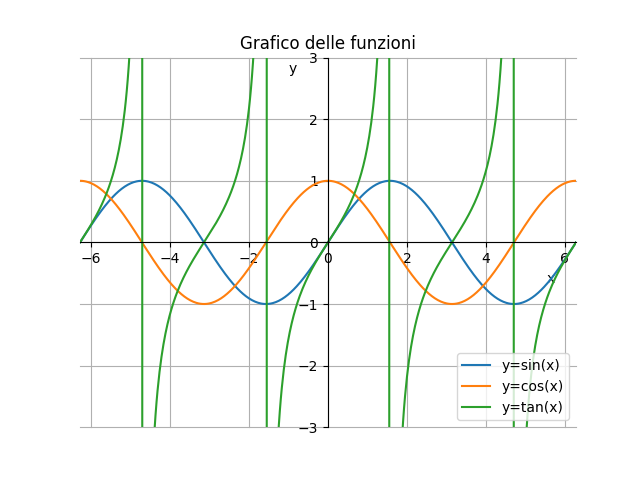
\includegraphics[width=1\textwidth]{images/trigonometriche.png}
  \caption{Funzioni trigonometriche}
\end{figure}

\end{document}

